\noindent \textbf{Part 1: Social Network Modeling} \\

\noindent This part is intended to get you started on the
project. \textbf{You may work with your project teammates and submit
	the same solution for this part only.} \\

\noindent Refer to the specification of the \textsf{Nicebook} social
network provided for the course project (\textsf{Social Network
	Spec.pdf}). Consider the description under the section \textbf{Basic
	Concepts} only (i.e., disregard operations or privacy settings for
this homework). 

\begin{enumerate}
	\item Construct an object model diagram for the social network.
	      
	      You may use any drawing tool of your choice and include the graphics
	      file as a figure in LaTeX\footnote{One freely available is Google
		      Drawings: \url{https://docs.google.com/drawings}}. Alternatively, it is acceptable to draw
	      the diagram by hand as long as it is legible.

        \textbf {Answer:}\\\\
        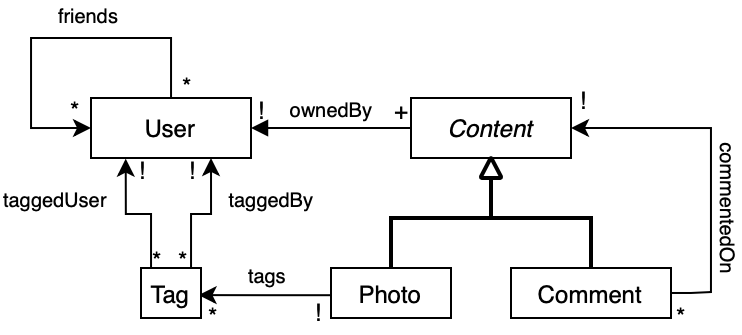
\includegraphics[width=5in]{hw6model.png}

	\item List at least one constraint from the above problem description that cannot be
	      expressed on this diagram.

        \textbf {Answer:} The following are the constraints that cannot be expressed on the object model diagram
            \begin {enumerate}
                \item $ \forall a, b: User \bullet b \in a.friends \implies a \in b.friends $\\
(If $a$ and $b$ are users then $a$ is friend of $b$ implies $b$ is friend of $a$)
                \item $ \forall a : User \bullet a \notin a.friends $\\
                    (If $a$ is a user then $a$ cannot be friend of $a$)
                \item $ \forall a : User \bullet \forall t : taggedUser.a \bullet t.taggedBy \subseteq t.friends $ \\
                    (If $a$ is a user then $a$ can only be tagged by $a$’s friends)
            \end {enumerate}
	\item Construct an Alloy model for this system. Your model must
	      include:
	      \begin{itemize}
		      \item A set of signatures and relations, but not operations or
		            privacy settings.
		      \item A predicate called \texttt{invariants} that defines the
		            set of constraints that every valid instance of the model must satisfy.
		      \item A \texttt{run} command called \texttt{GenerateValidInstance} that generates only valid instances.
	      \end{itemize}
	      Name your model file \texttt{hw6-1.als}  and submit it on
	      Canvas. In addition, include a copy of your Alloy model in your
	      Gradescope submission. 

          \smallskip \textbf{Answer:} 
          \begin{alloy}
/****************
 * SIGNATURES
 ****************/

sig User {
	friends : set User
}

abstract sig Content {
	ownedBy : one User,
}

sig Photo extends Content {
    tags : set Tag  // Can tag 0 or more User
}

sig Comment extends Content {
	commentedOn : one Content // Can comment on only one Content
}

sig Tag {
    taggedUser : one User,
    taggedBy : one User
}

/****************
 * INVARIANTS 
 ****************/

-- User cannot be a friend of itself
pred invariantNoUserCanBeFriendsWithSelf {
	all u : User | u not in u.friends // Note: Loops are allowed though
}

-- If a and b are users then a is friend of b implies b is friend of a
pred invariantFriendsAreCommutative {
	all u1, u2 : User | u1 in u2.friends implies u2 in u1.friends
}

-- Users can only be tagged by their friends
pred invariantUsersCanBeTaggedByFriendsOnly {
	all  t: Tag | t.taggedBy in t.taggedUser.friends
}

-- User owns one or more content
pred invariantUserOwnsAtleastOneContent {
	all u : User | u in Content.ownedBy
}

-- Same user cannot be tagged twice in a photo
pred invariantCannotTagSameUserInOnePhoto {
	all t1, t2: Tag | t1 != t2 implies t1.taggedUser != t2.taggedUser 
}

-- if there is a tag, it must be correlated with exactly one photo
pred invariantTagIsAssociatedWithExactlyOnePhoto {
	all t : Tag | one tags.t
}

-- Additional --

-- Comments cannot be dangling, last comment should be attached to content
pred invariantCommentCannotBeDangling {
	all com : Comment | (some p : Photo | p in com.^commentedOn)
}

-- Comments should not have cycles
pred invariantCommentsCannotHaveCycles {
	all com : Comment | com not in com.^commentedOn
}

pred Invariants {
	invariantNoUserCanBeFriendsWithSelf
	invariantFriendsAreCommutative
	invariantUsersCanBeTaggedByFriendsOnly
	invariantUserOwnsAtleastOneContent
	invariantCannotTagSameUserInOnePhoto
	invariantTagIsAssociatedWithExactlyOnePhoto
	invariantCommentsCannotHaveCycles
	invariantCommentCannotBeDangling
}

/****************
 * RUN 
 ****************/

run GenerateValidInstance {
	Invariants
}
          \end{alloy}
\end{enumerate}
